\documentclass{stdlocal}
\begin{document}
\section{Evaluation and Results} % (fold)
\label{sec:evaluation}
  \autocite{compiler-explorer,intel-intrinsics-guide,perfevent,vandevoorde2018,meyers2014}

  In section \ref{sec:implementation}, we have implemented scalar and vectorized versions of known PRNGs, namely the MT19937, the Xoroshiro128+, and the MSWS.
  Additionally, unbiased uniform distribution functions for floating-point numbers based on \textcite[\ppno~55-56]{kneusel2018} and \textcite{vigna-xoroshiro} were introduced to completely exploit the vector registers as long as possible.
  The last section \ref{sec:testing_framework} described the implementation of tests and benchmarks to measure the performance of PRNGs concerning statistics and execution time.
  So to prove that the vectorization of PRNGs is indeed improving the performance without reducing statistical quality, we have to apply those benchmarks and analyze their output.

  We have run the benchmarks on two different machines with similar architectures with varying raw computing powers.
  The machines are modern Linux-based $64\appendUnit{bit}$ platforms providing the GCC C++ compiler version 9.2.0 \autocite{gcc}.
  The given C++ code used for including the library and running the tests and benchmarks was compiled with the optimization flags \code{-O3} and \code{-march=native} to guarantee the strongest optimization level.
  Because the generation of random numbers through PRNGs typically does not have to access main memory and can instead completely be run inside the caches of the CPU, specifying the CPU parameters of a target machine will be sufficient to draw conclusions.
  The first machine is a laptop and consists of the \citetitle{intel-kaby-lake-i5} \autocite{intel-kaby-lake-i5} whereas the second machine is a custom desktop computer with an installed \citetitle{intel-kaby-lake-i7} \autocite{intel-kaby-lake-i7}.
  Both systems consist of four cores featuring Hyper-Threading and the SSE/AVX instruction set extensions up to SSE4.2 and AVX2.
  The desktop processor is an high-end performance microprocessor based on the Kaby Lake microarchitecture.
  It operates at a base frequency of $4.2\appendUnit{GHz}$ and a Turbo Boost frequency of up to $4.5\appendUnit{GHz}$ when used in single-core mode.
  The laptop processor is a mobile microprocessor and is also based on an enhanced version of the Kaby Lake microarchitecture.
  It operates at a base frequency of $1.6\appendUnit{GHz}$ and a Turbo Boost frequency of up to $3.4\appendUnit{GHz}$.
  We refer to \textcite{intel-kaby-lake-i5} and \textcite{intel-kaby-lake-i7} for more information.

  \subsection{Statistical Quality} % (fold)
  \label{sub:statistical_quality}
    From a theoretical point of view, interleaving multiple streams of random numbers based on multiple instances of the same generator should not reduce the randomness of the output, such that test suites will be able to measure it.
    Using multiple instances through SSE/AVX vector registers the state of the vectorized PRNG becomes at least two times as big as the scalar variant.
    According to \textcite{oneill-blog-toobig}, creating a larger state will even make a weak generator stronger concerning its statistical performance.
    On the other hand, \textcite{fog2015} states that the use of multiple instances of the same generator with different seeds can lead to overlapping subsequences.

    For testing the statistical performance, we have used TestU01 version 1.2.3 and version 3.31.1 of dieharder.
    The computation time to run all the tests in the test batteries of TestU01 approximately ranged from $5\appendUnit{s}$ for SmallCrush over $20\appendUnit{min}$ for Crush to $150\appendUnit{min}$ for BigCrush.
    While executing the BigCrush battery, 160 statistics were used to estimate the statistical performance of the generators.
    The execution of all 30 dieharder tests with different parameters always took several minutes.

    Running the statistical test suites, we could not find any vulnerabilities.
    Neither the scalar nor the vectorized versions of the Xoroshiro128+ and the MSWS systematically failed an empirical test.
    Even a truly random sequence will fail tests from time to time \autocite[\pno~142]{kneusel2018} and so after running the test suites multiple times, we wer able to confirm this for our implementations, too.
    Every generator rarely produced test failures that did not follow any pattern.
    We conclude that the usage of multiple instances to vectorize the generators did not reduce their statistical quality.
  % subsection statistical_quality (end)

  \subsection{Performance Improvement} % (fold)
  \label{sub:performance_improvement}

    \begin{figure}
      \center
      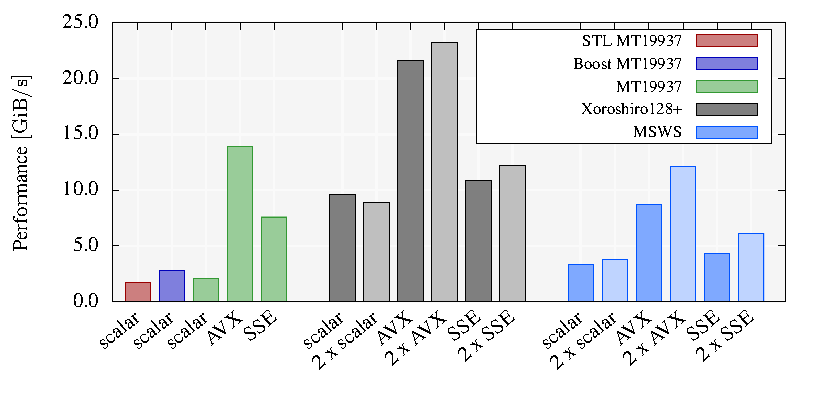
\includegraphics[width=0.95\textwidth]{plots/generation_desktop.pdf}
      \caption[Generation Benchmark Performance for \citetitle{intel-kaby-lake-i7}]{%
        The plot shows the performance resulting from the generation benchmark running on the \citetitle{intel-kaby-lake-i7} measured in $\mathrm{GiB}$ of random numbers per second for the different variants of the implemented PRNGs.
        % The prefix \enquote{2 x} states that two independent instances of the given generator were used.
        For convenience, the performances of the STL and Boost implementation of the MT19937 are shown as well.
        The data can be found in table \ref{tab:generation-data-i7}.
      }
    \end{figure}

    \begin{figure}
      \center
      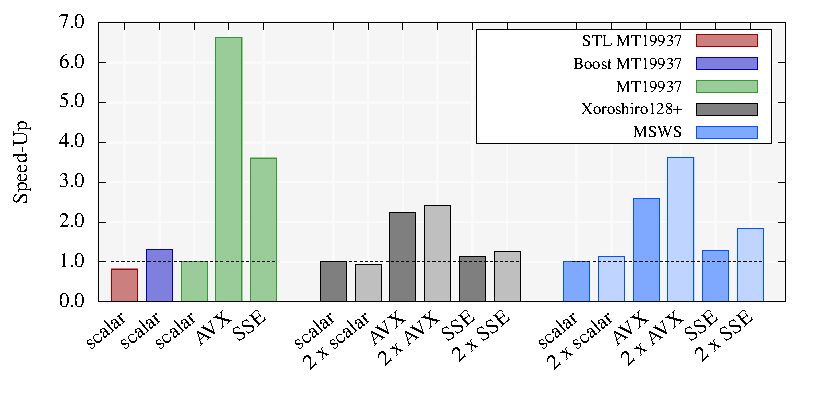
\includegraphics[width=0.95\textwidth]{plots/generation_desktop_speedup.pdf}
      \caption[Generation Benchmark Speed-Up for \citetitle{intel-kaby-lake-i7}]{%
        The plot shows the speed-up in execution time with respect to the single-instance scalar version resulting from the generation benchmark running on the \citetitle{intel-kaby-lake-i7} for the different variants of the implemented PRNGs.
        For convenience, the speed-ups of the STL and Boost implementation of the MT19937 are shown with respect to our implementation.
        The data can be found in table \ref{tab:generation-data-i7}.
      }
    \end{figure}

    \begin{table}
      \center
      \caption[Generation Benchmark Data for \citetitle{intel-kaby-lake-i7}]{%
        The table shows the results achieved by running the generation benchmark on the \citetitle{intel-kaby-lake-i7} at a frequency of $4.51\appendUnit{GHz}$ with all implemented variants of given PRNGs.
        While running the benchmark, $16\appendUnit{GiB}$ of random numbers were generated and temporarily stored in a cache of size $16384\appendUnit{B}$ by iterating $2^{20}$ times over its content.
        During the execution, there were no cache or branch misses.
        The values for cycles, instructions, and IPCs were averaged over the calls to the advancing routine of the respective generator.
      }
      \label{tab:generation-data-i7}
      \footnotesize
      \renewcommand{\arraystretch}{1.2}
      \subimport{tables/}{generation_desktop}
    \end{table}

    \begin{figure}
      \center
      \begin{subfigure}[b]{\textwidth}
        \center
        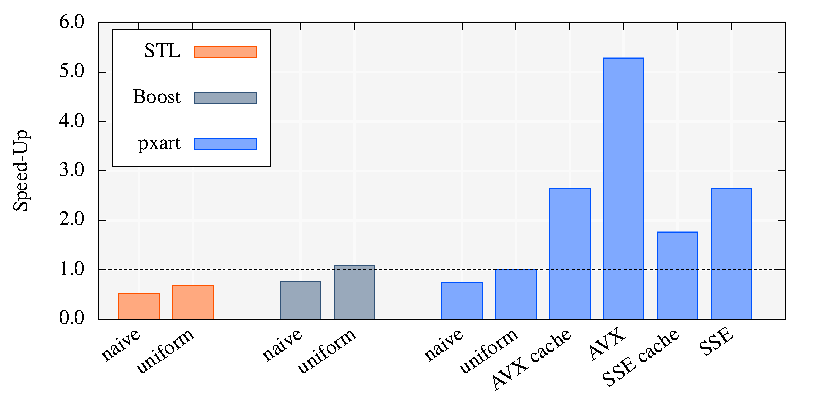
\includegraphics[width=0.95\textwidth]{plots/monte_carlo_pi_desktop_mt19937.pdf}
        \caption{MT19937}
      \end{subfigure}

      \begin{subfigure}[b]{\textwidth}
        \center
        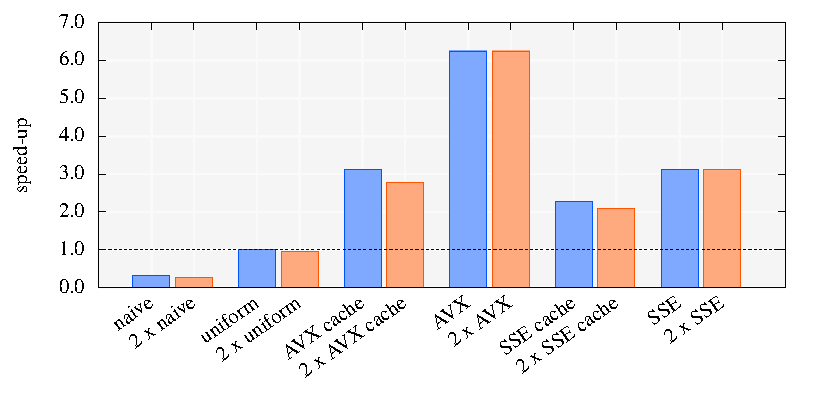
\includegraphics[width=0.95\textwidth]{plots/monte_carlo_pi_desktop_xrsr128p.pdf}
        \caption{Xoroshiro128+}
      \end{subfigure}

      \begin{subfigure}[b]{\textwidth}
        \center
        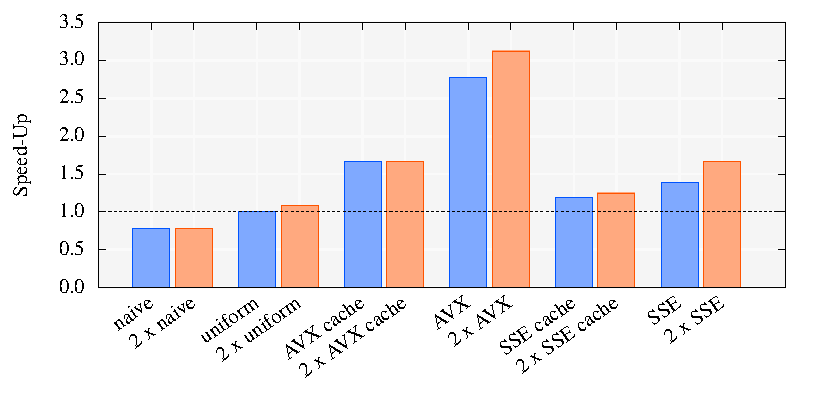
\includegraphics[width=0.95\textwidth]{plots/monte_carlo_pi_desktop_msws.pdf}
        \caption{MSWS}
      \end{subfigure}
      \caption[Monte Carlo π Benchmark Speed-Up for \citetitle{intel-kaby-lake-i7}]{%
        The plot shows the speed-up in execution time with respect to the single-instance uniform version resulting from the Monte Carlo π benchmark running on the \citetitle{intel-kaby-lake-i7} for the different variants of the implemented PRNGs and benchmark scenarios.
        For convenience, the speed-ups of the STL and Boost implementation of the MT19937 are shown with respect to our implementation.
        The data can be found in table \ref{tab:monte-carlo-pi-data-i7}.
      }
    \end{figure}

    \begin{table}
      \center
      \caption[Monte Carlo π Benchmark Data for \citetitle{intel-kaby-lake-i7}]{%
        The table shows the results achieved by running the Monte Carlo π Benchmark on the \citetitle{intel-kaby-lake-i7} with all implemented variants of given PRNGs and benchmark scenarios.
        While running the benchmark, $10^{8}$ samples in the unit square were used to estimate the value of π.
        It was ensured that the estimation error was small enough according to the calculation at the end of section \ref{sub:monte_carlo_integration}.
        During the execution, there were no cache or branch misses.
        The values for cycles, instructions, and IPCs were averaged over the number of samples in the unit square.
      }
      \label{tab:monte-carlo-pi-data-i7}
      \footnotesize
      \renewcommand{\arraystretch}{1.2}
      \subimport{tables/}{monte_carlo_pi_desktop.tex}
    \end{table}

  % subsection performance_improvement (end)
% section evaluation (end)
\end{document}